\scanpage{7}
\mspage{2}

comme l'unique élément de \({}_2(X_S)\) qui est fixe par $\operatorname{Aut}(X_S)\simeq\mathbb Z/4\mathbb Z$. En fait
\inserted{\[
(X_S)^{\unsure{\deleted{i}|f}i}\overset{\mathrm{def}}{=}\{x\in X_S\deleted{\}} \mid ix\unsure{=|\simeq}x\}=\{e,\eta_S\}
\]}
\deleted{\unsure{$X$|$X_S$}} La surface top. $X_S$ a une déc. cell. \inserted{\unsure{can|ces}} avec 1 sommet $e$, deux arêtes, une face, \inserted{ces arêtes} correspondant aux deux mailles du réseau $\Gamma_S$.

On considère $X_S$ comme muni de cette décomposition. Parfois c'est l'image inv. de celle-ci par $2\operatorname{id}_{X_S}$ qui est plus commode, 4 sommets (formant \({}_2(X_S)\)), \deleted{quatre} \inserted{huit} arêtes, \deleted{(\uline{NB} \unsure{le}} \inserted{$4^{\unsure{\smallfrown}}$} faces. On peut considérer $\mathbb Z/4\mathbb Z\simeq\mu_4(\mathbb C)$ comme le groupe d'automorphismes commun de ces deux structures cellulaires.

\figure{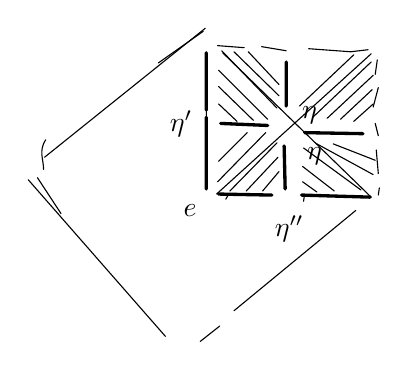
\begin{tikzpicture}[x=.013cm,y=-.013cm,line cap=round,line join=round]
\draw[thin] (-153,110)--(4,-16);
\draw[thin] (-152,93) .. controls (-159,104) and (-154,112) .. (-154,122);
\draw (-42,18)--(2,-13);
\draw (-169,132)--(-35,285);
\draw (-160,130)--(-137,165);
\draw[thin] (32,260)--(151,162);
\draw[thin] (-1,290)--(18,275);
\draw[thin] (21,8)--(166,149) (166,9)--(15,146);
\draw[thin] (20,6)--(74,62) (32,7)--(76,50) (46,7)--(76,39)
 (17,25)--(65,73) (17,41)--(51,74) (17,58)--(35,75);
\draw[thin] (96,60)--(149,10) (109,71)--(166,17)
 (123,72)--(168,30) (136,73)--(167,44) (149,75)--(168,58);
\draw[thin] (16,134)--(63,86) (28,143)--(74,96)
 (44,143)--(75,110) (60,143)--(76,124) (17,114)--(45,86);
\draw[thin] (100,101)--(156,142) (113,97)--(168,127)
 (129,97)--(170,113) (99,119)--(130,143) (99,134)--(113,144);
\draw (16,1)--(42,3) (59,2)--(83,6) (105,4)--(146,7)--(163,5);
\draw (172,15)--(170,29) (173,42)--(168,61) (170,77)--(173,89)
 (171,103)--(173,126) (174,140)--(173,147);
\draw[line width=1.2pt] (5,8)--(5,64) (5,71)--(5,141)
 (17,146)--(69,147) (98,147)--(165,149)
 (83,17)--(83,60) (81,99)--(82,141)
 (19,77)--(65,79) (101,86)--(158,87);
\draw[thin] (5,64)--(5,71) (27,146)--(24,151) (101,146)--(100,153);
\node[below left] at (5,147) {$e$};
\node[left] at (1,77) {$\eta'$};
\node[below] at (86,158) {$\eta''$};
\node[above right] at (89,87) {$\eta$};
\node[below right] at (94,91) {$\deleted{\unsure{\eta}}$};
\end{tikzpicture}}

Le deuxième est mieux \unsure{adaptée|adapté} pour la description du quotient
\[
\deleted{\unsure{X}\mathbb E\unsure{\ell_0|\ell}(\unsure{S|8})}\quad X_S/\pm1
\]
qui est une sphère, subdivisée en \deleted{deux} \inserted{faces} carrées, se raccordant suivant un équateur \deleted{carré}. subdivisé en quatre arêtes par $e^\natural,\eta^\natural,\eta'^\natural,\eta''^\natural$.

\figure{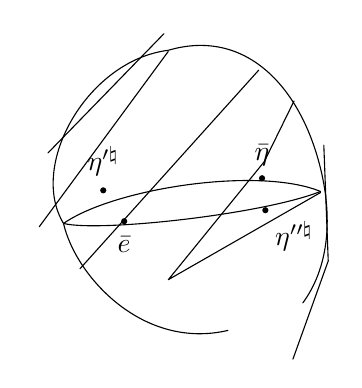
\begin{tikzpicture}[x=.014cm,y=-.014cm,line cap=round,line join=round]
\draw (34,182) .. controls (2,129) and (56,34) .. (129,25)
 .. controls (197,5) and (248,55) .. (267,132)
 .. controls (279,181) and (273,224) .. (251,254);
\draw (34,182) .. controls (45,230) and (106,297) .. (183,279);
\draw (34,182) .. controls (80,150) and (211,130) .. (267,153);
\draw (34,182) .. controls (66,190) and (214,174) .. (267,153);
\fill (70,152) circle (2.8);
\fill (214,141) circle (2.8);
\fill (89,180) circle (2.8);
\fill (217,170) circle (2.8);
\node[above] at (70,148) {$\unsure{\eta'^\natural}$};
\node[above] at (214,139) {$\bar\eta$};
\node[below] at (89,185) {$\bar e$};
\node[below right] at (217,172) {$\unsure{\eta''^\natural}$};
\draw (20,118)--(125,10) (12,185)--(129,26)
 (49,223)--(211,43);
\draw (243,71)--(216,126)--(129,233)--(267,154);
\draw (242,305)--(274,216)--(270,111);
\end{tikzpicture}}
\figure{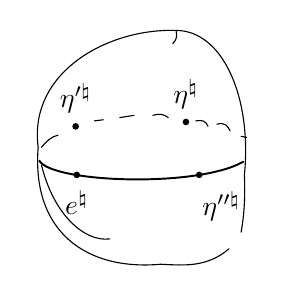
\begin{tikzpicture}[x=.014cm,y=-.014cm,line cap=round,line join=round]
\draw (14,126) .. controls (5,58) and (77,18) .. (139,20)
 .. controls (181,20) and (208,80) .. (201,151)
 .. controls (202,177) and (200,191) .. (198,203);
\draw (187,218) .. controls (167,235) and (147,233) .. (125,232)
 .. controls (57,238) and (8,202) .. (14,126);
\draw (17,126) .. controls (21,121) and (26,116) .. (32,115);
\draw (65,102)--(73,101) (88,99)--(101,97);
\draw (118,97) .. controls (124,95) and (128,96) .. (132,99);
\draw (157,102) .. controls (163,101) and (166,102) .. (168,107);
\draw (176,105) .. controls (184,103) and (186,107) .. (188,111);
\draw (198,116)--(203,117);
\draw[line width=.7pt] (15,138) .. controls (26,158) and (158,163) .. (200,139);
\draw[thin] (139,20) .. controls (140,25) and (140,28) .. (136,32);
\draw[thin] (17,142) .. controls (28,187) and (56,212) .. (79,209);
\fill (48,107) circle (3);
\fill (148,103) circle (3);
\fill (49,151) circle (3);
\fill (160,151) circle (3);
\node[above] at (48,104) {$\eta'^\natural$};
\node[above] at (148,100) {$\eta^\natural$};
\node[below] at (49,157) {$e^\natural$};
\node[below right] at (154,158) {$\eta''^\natural$};
\end{tikzpicture}}

\margin{6}

